\documentclass[10pt,aspectratio=43]{beamer}
\usepackage{bibentry}
\usepackage[style=bwl-FU]{biblatex}
\usepackage[dvipsnames]{xcolor}
\usepackage{graphicx} % Allows including images
\usepackage{booktabs} % Allows the use of \toprule, 
\usepackage{array}
\usepackage{wrapfig}
\usepackage{graphics}
\usepackage{graphicx}
\usepackage{amsfonts}
\usepackage{amssymb}
\usepackage{amsthm}
\usepackage{textcomp}
% \usepackage{enumitem}
\usepackage{graphicx} % Allows including images
\usepackage{booktabs} % Allows the use of \toprule, 
% \usepackage[nottoc]{tocbibind}
\usepackage{threeparttable}
% \usepackage{natbib}
% \usetheme{SimpleDarkBlue}

% \usepackage{mathrsfs}
\usepackage[nospace]{varioref}	
\usepackage{cleveref}

\usepackage{presentation}

\setlength{\parskip}{\baselineskip} 
% \graphicspath{{./../Figures}}
% \setlength\itemsep{2em}

\setlength\belowcaptionskip{-3ex}


\usepackage{caption}
\usepackage{subcaption}

\bibliography{references.bib}


\usepackage{makecell}

% \usecolortheme{}
\usepackage{amsmath}


\DeclareMathOperator*{\argmax}{arg\,max}
\DeclareMathOperator*{\argmin}{arg\,min}


\title{Bayesian Estimation of Risk-Neutral Probability}
% Enter presentation information:
\information%
% Enter link to research paper (optional; comment line if not needed):
%[]%
% Enter presentation authors:
{Alexander Vlasov (avlasov@nes.ru)}%
% Enter presentation location and date (optional; comment line if not needed):
{New Economic School -- 2025-06-20}

% \usecolortheme{}

% \AtBeginSection{
% 	\begin{frame}[fragile]\Large	
% 		\frametitle{Contents}
% 		\tableofcontents[currentsection]
% 	\end{frame}
% }
% \setbeamerfont{footnote}{size=\tiny}


% \setbeamerfont{normal text}{size=\small}
% \AtBeginDocument{\usebeamerfont{normal text}}


\graphicspath{{../Figures/}}

\begin{document}

\begin{frame}[fragile]
    \titlepage
\end{frame}



% \section{Limitations of RA models}
% \begin{frame}[fragile]{Contents}
%     \large
%     \tableofcontents[currentsection]
% \end{frame}

\begin{frame}{\al{Implied} Risk-Neutral Probability Density (State-Price Density)}

    \[S=\sum_{s=1}^K\phi(s)q(s)\]

    \[\phi^*\overset{d}{=}\frac{\phi(s)}{\sum_{s=1}^K\phi(s)}=\frac{\phi(s)}{1/(1+r)}=(1+r)\phi(s)\]

    \[S=\frac{1}{1+r}\sum_{s=1}^K\phi^*(s)q(s)=\frac{1}{1+r}\mathbb{E}^*[q(s)].\]

\end{frame}
\begin{frame}{Implied \al{Risk-Neutral} Probability Density}
 
    For TAS utility, the state-prices are 
    \[\phi(s)=\pi\frac{\beta u'[c(s)]}{u'[c(0)]},\]
    \then implied risk-neutral probability is
    \[\phi^*(s)=\pi\frac{\beta u'[c(s)]}{u'[c(0)]}(1+r)= \pi\frac{u'[c(s)]}{u'[c(0)]}\approx \pi,\]
    for $u'$ is constant (risk-neutrality) or $c(s)\approx c(0)~\forall s$.


\end{frame}


\begin{frame}{Approaches to Estimation}
    \begin{itemize}  \setlength\itemsep{1em}
        \item Estimation of $C$ with shape restrictions -- $C^2$ approximation with 2nd derivative being a valid density \\{\scriptsize\parencite{ait-sahaliaNonparametricOptionPricing2003}}
        \item Bayesian methods \\{\scriptsize\parencite{fisherSimplexRegression2016, hardleStatePriceDensities2015,tabogaOptionimpliedProbabilityDistributions2016} + KDE in the second case}
        \item 
    \end{itemize}
\end{frame}

\begin{frame}{Breeden-Litzenberger (1978) Formula}
\nocite{breedenPricesStateContingentClaims1978}
For short-term, $r\approx 0$.
    \begin{align*}
        C(S,t)&=\mathbb{E}^*\left[[S(T)-\mathcal{K}]^+\mid S(t)=S\right]\\ 
        &=\int_0^{+\infty}(x-\mathcal{K})^+\,dP^*(x)\\ &=\int_{\mathcal{K}}^{+\infty}x\,dP^*(x)-\mathcal{K}\int_0^{+\infty}\,dP^*(x)\\ 
        &=\int_{\mathcal{K}}^{+\infty}x\,dP^*(x)-\mathcal{K}(1-P^*(\mathcal{K}))
    \end{align*}
    \begin{align*}
        \frac{\partial C}{\partial \mathcal{K}}&=-\mathcal{K}p^*(\mathcal{K})-1+P^*(\mathcal{K})+\mathcal{K}p^*(\mathcal{K})=P^*(\mathcal{K})-1\\ 
        \frac{\partial^2 C}{\partial \mathcal{K}^2}&=p^*(\mathcal{K}).
    \end{align*}
   We need an option price, $C$, to be twice differentiable, $C^2$, function. 
\end{frame}


\begin{frame}{Bayesian Formulation}
    \cite{fisherSimplexRegression2016} proposes the following approach.\footnote[frame]{\tiny This is the methodology for \cite{MarketProbabilityTracker}.}
\vspace{-2ex}
    \[y_i=\lambda\sum_{j=1}^KX_{ij}\beta_j+\varepsilon_i,\]
    where $\beta=(\beta_1,\dots, \beta_K)\in \Delta^{K-1}$, $\Delta^{K-1}$ denotes the simplex of dimension $(K-1)$; $X_{ij}$ is a payoff of derivative $i$ in state $j$, and $\varepsilon_i\sim N(0,\sigma^2)$.

    In vector form,
    \[y=\lambda X \beta+\varepsilon.\]

\vspace{-2ex}
    In order to insure $\beta\in \Delta^{K-1}$, we select the (symmetric) Dirichlet prior:
    \[p(\beta\mid \alpha)=\operatorname{Dirichlet}(\beta\mid \alpha)\propto \prod_{i=1}^{K}x_{i}^{\alpha-1}.\]

\end{frame}

\begin{frame}{}
$X$ consists of $n$ payoffs of $K$ derivatives, including the payoffs price (you can think of it as call option with strike equal zero).

The state space is chosen to ensure that the first and last coefficients are near zero, so the list of possibilities is exhaustive.
 \begin{figure}\centering
    \begin{minipage}{0.6\linewidth}
        \centering
                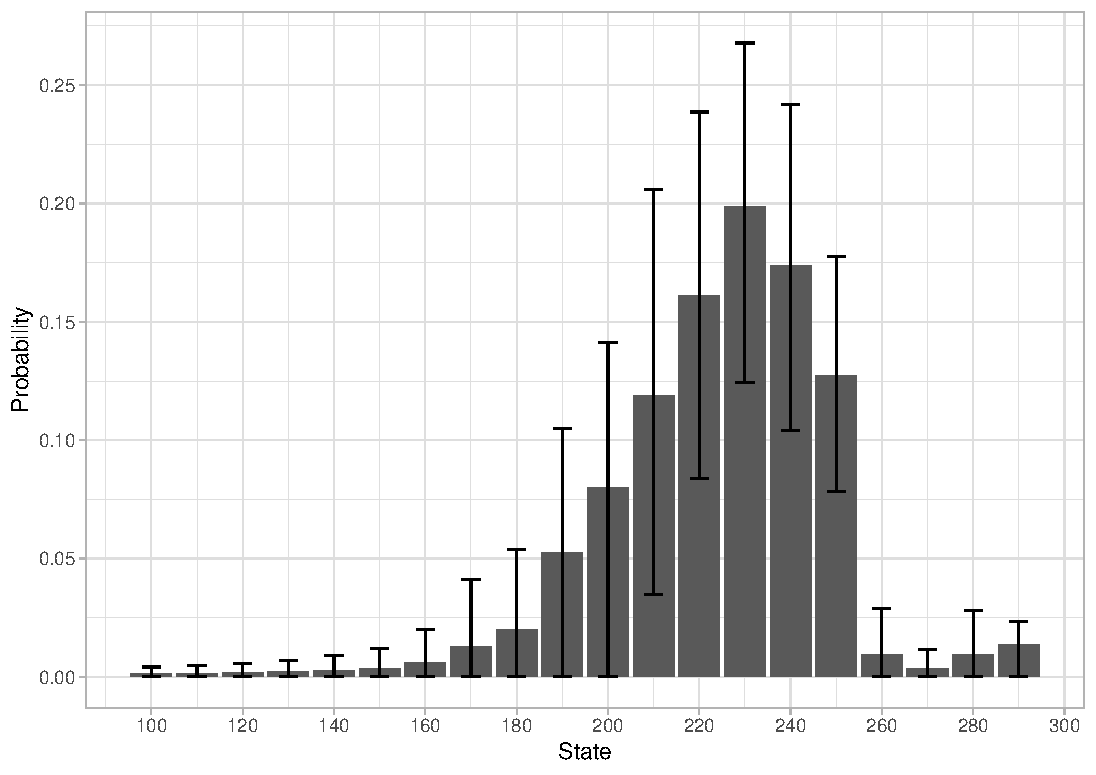
\includegraphics[width=\linewidth]{betas_01_3.pdf}
    \end{minipage}
    \end{figure}

\end{frame}

\begin{frame}{Prior for Concentration Coefficient}
    $\alpha$ is a vector of concentration parameters for Dirichlet distribution. The lower the value, the less 'flat' the distribution of risk-neutral density $\beta$.
    
    It is reasonable to select a distribution that is relatively flat on $[0,1]$ and assign a large portion of mass to $[0,1]$. \cite{fisherSimplexRegression2016} uses Lognormal prior, I propose Weibull. The result turns out to be almost identical.

    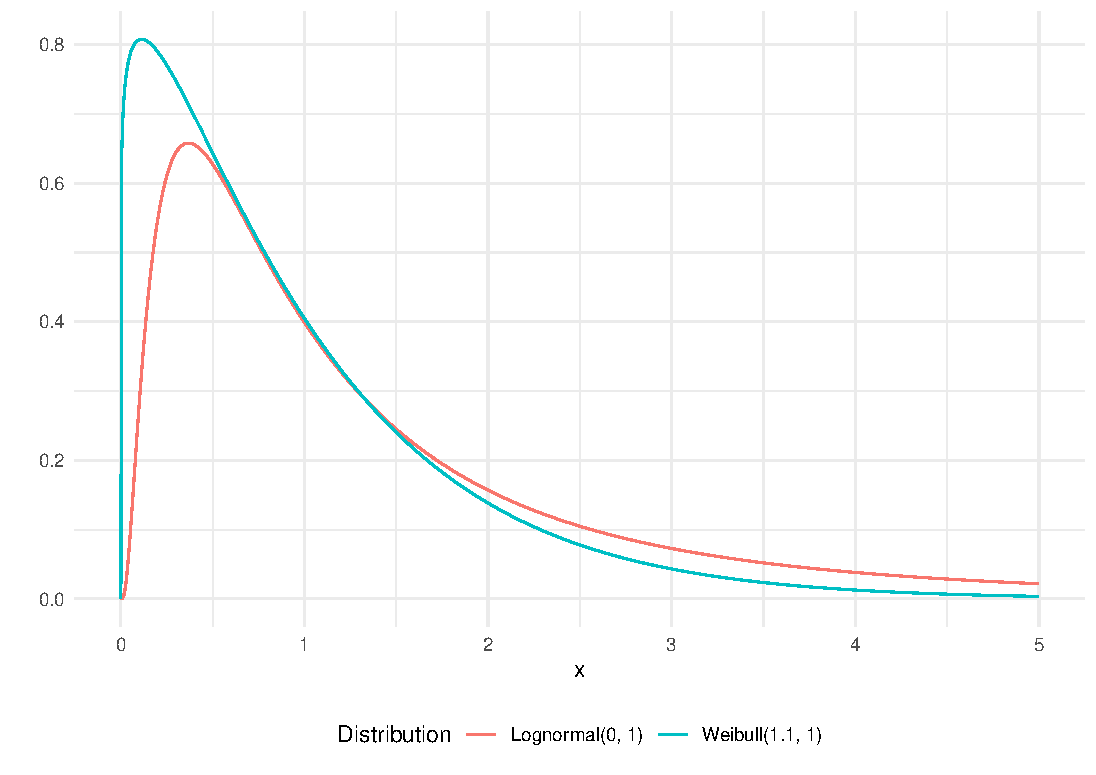
\includegraphics[width=0.6\textwidth]{prior_difference.pdf}

\end{frame}

\begin{frame}{Priors and Posterior}
     \[p(\beta\mid \alpha)=\operatorname{Dirichlet}(\beta\mid \alpha)\propto \prod_{i=1}^{K}x_{i}^{\alpha-1}.\]
    \[p(\alpha)=\operatorname{Weibull}(1.1,1)\]
    \[p(\sigma^2)\propto \frac{1}{\sigma^2}\]

    \[p(\alpha,\lambda,\sigma,\beta\mid y)\propto N(y\mid \lambda X\beta,\sigma)\times\operatorname{Dirichlet}(\beta\mid \alpha)\times \operatorname{Weibull}(1.1,1)\times \frac{1}{\sigma^2}\]

\end{frame}





\begin{frame}{Risk Neutral Density for AAPL I}
    Calculated in 2025-04-01 with expiration date 2025-04-17 (\al{+16 days}). Wiskers are 90\% HPD interval.
     \begin{figure}\centering
        \begin{minipage}{0.75\linewidth}
        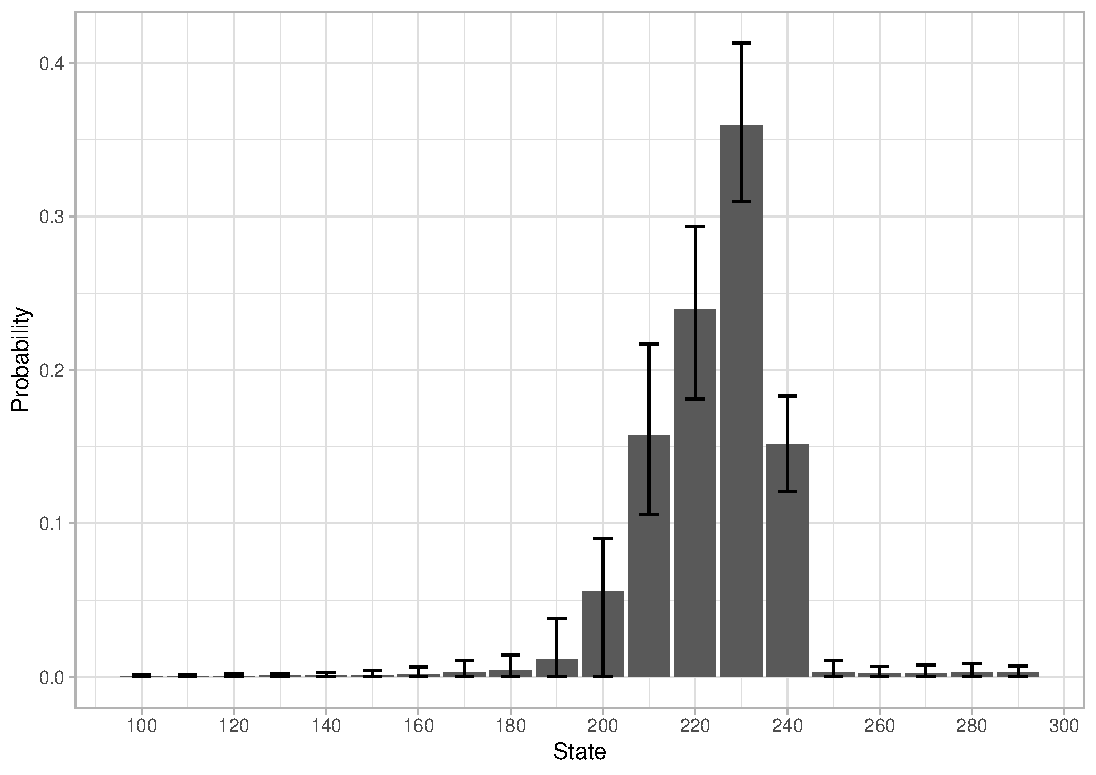
\includegraphics[width=\linewidth]{betas_01_1.pdf}
     \end{minipage}
    \end{figure}
\end{frame}

\begin{frame}{Risk Neutral Density for AAPL II}
    Calculated in 2025-04-01 (same) with expiration date 2025-05-16 (\al{+45 days}).
    \begin{figure}\centering
        \begin{minipage}{0.75\linewidth}
        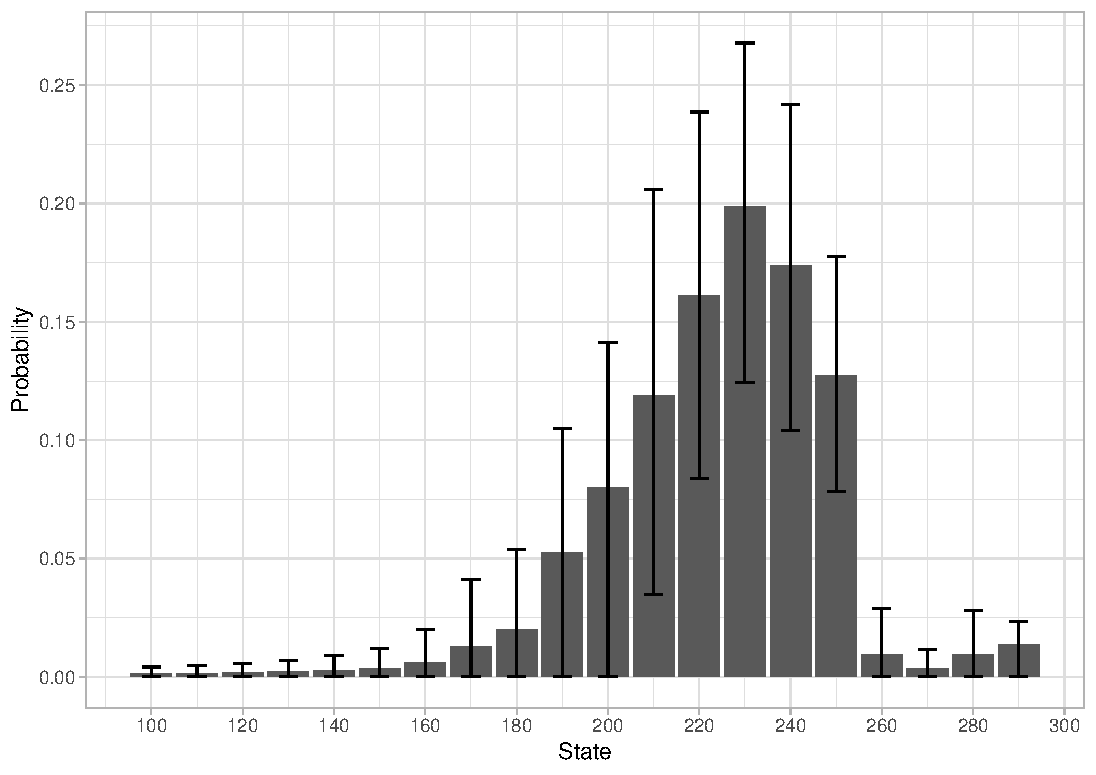
\includegraphics[width=\linewidth]{betas_01_3.pdf}
     \end{minipage}
    \end{figure}
\end{frame}



\begin{frame}{Density before and after the ``Liberation Day'' 2025-04-02}
    \begin{figure} \centering
        \begin{minipage}{0.9\linewidth}
                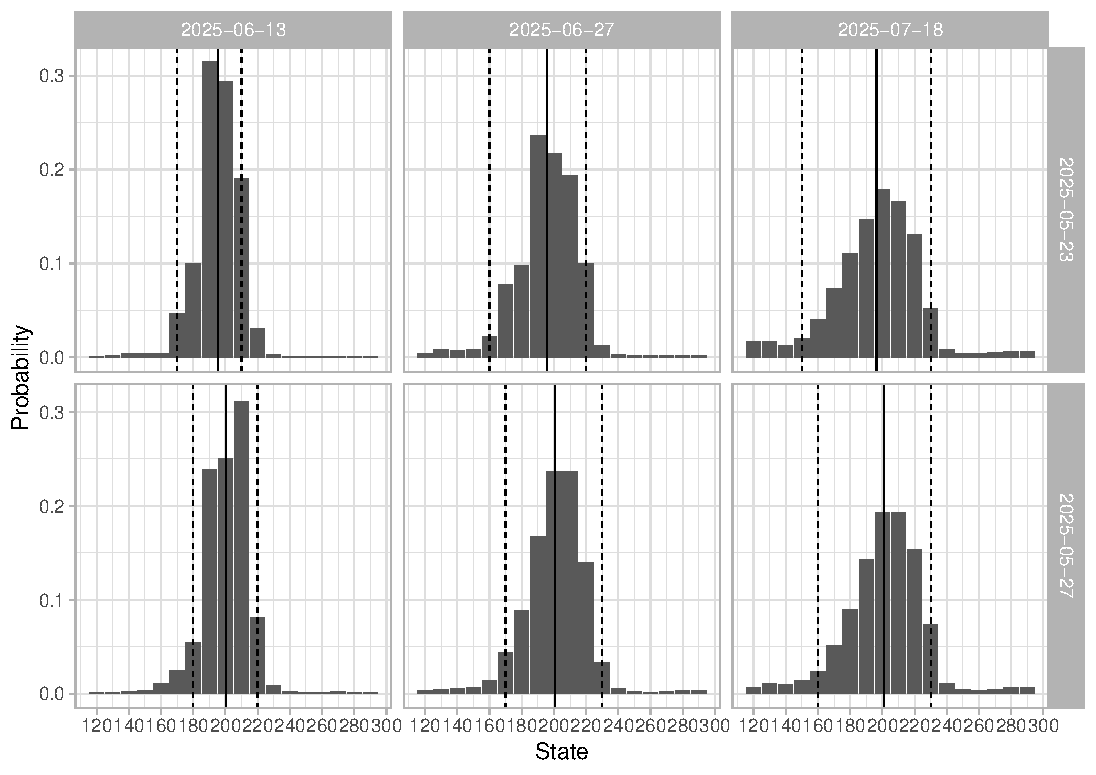
\includegraphics[width=\linewidth]{betas.pdf}
        \end{minipage}
    \end{figure}
\end{frame}
 

\begin{frame}{Summary Statistics \& Sanity Check}
    \begin{figure}\centering
        \begin{minipage}{0.9\linewidth}
            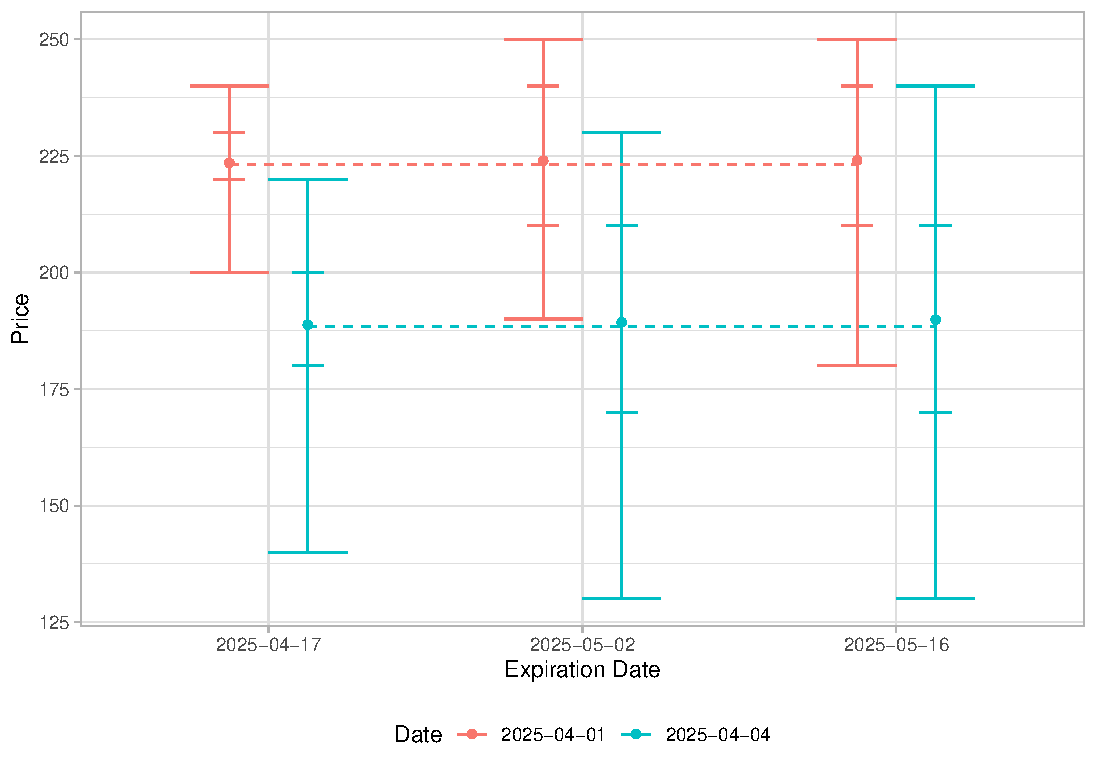
\includegraphics[width=\linewidth]{summaries_plot.pdf}
        \end{minipage}
    \end{figure}
\end{frame}


\begin{frame}{Concentration Parameter Posterior Distribution}

    Concentration parameter, $\alpha$, is a measure of uncertainty in the risk-neutral probability density. The lower the value, the less 'flat' the distribution, indicating lower uncertainty.

    \begin{figure}\centering 
        \begin{minipage}{0.7\linewidth}
            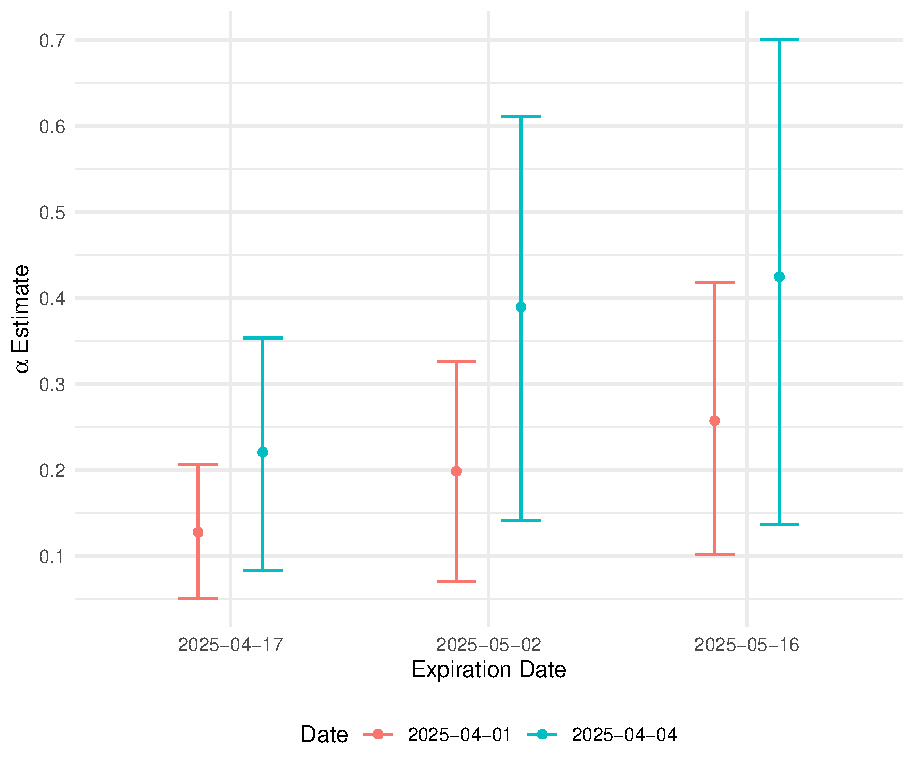
\includegraphics[width=\textwidth]{alphas.pdf}
        \end{minipage}
    \end{figure}
\end{frame}

\begin{frame}{Concentration Parameter Posterior Distribution}
    
    The posterior distribution of the concentration parameter, $\alpha$, for expiration 2025-04-17.
\begin{figure}
    \begin{minipage}{0.9\linewidth}
        \centering
        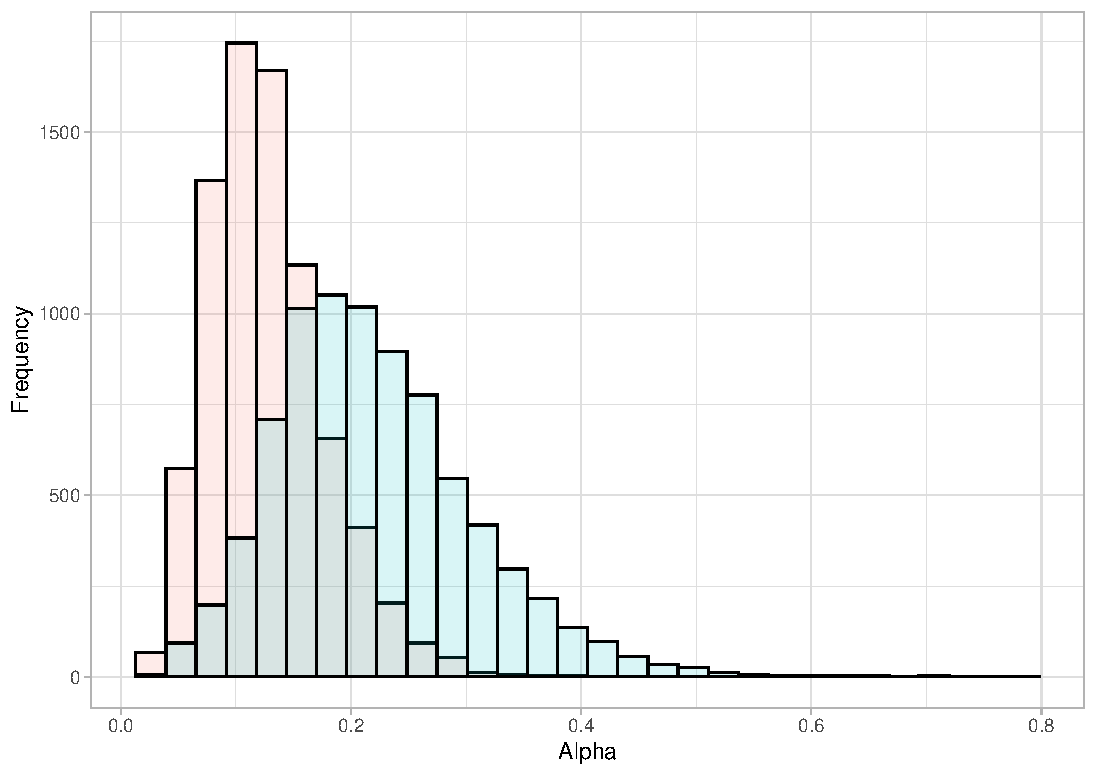
\includegraphics[width=0.8\linewidth]{alpha_histogram.pdf}
    \end{minipage}
\end{figure}
\end{frame}

\begin{frame}{Concentration Parameter and State Space}
    The concentration parameter is dependent on the state space. Since we want to ensure that the list of possibilities is exhaustive, we will be facing several betas close to zero. This corresponds to the concentration parameter being close to zero.
    \begin{figure}[htbp]
    \begin{minipage}{0.9\linewidth}
        \centering
        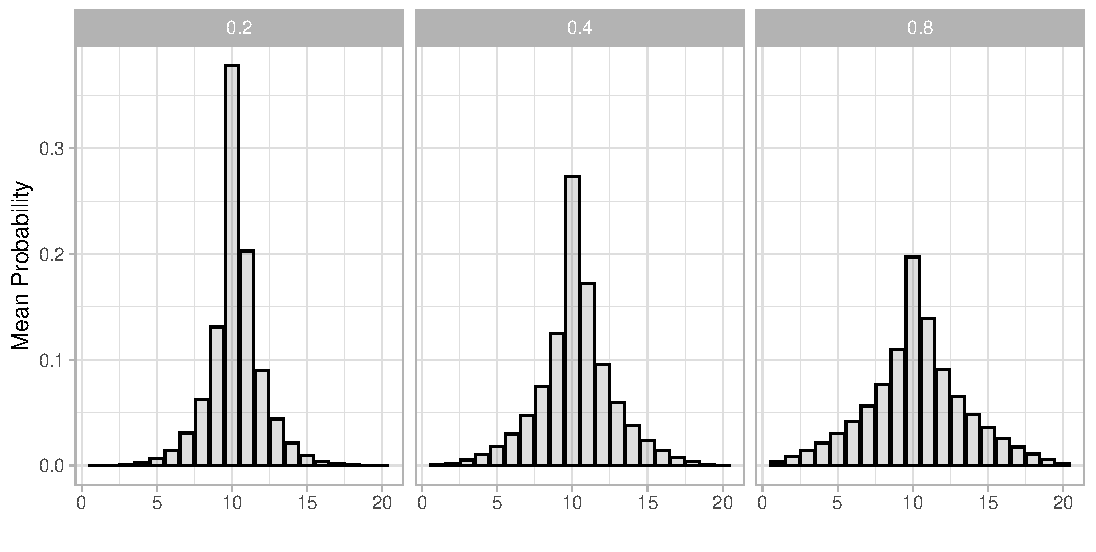
\includegraphics[width=\linewidth]{dirichlet_histogram.pdf}
        \vspace{-6ex}
        \begin{flushleft}
        \tiny \textit{Notes:} This figure shows the means of random samples from Dirichlet distribution, that are arranged in order to resample the distribution of state prices.
        \end{flushleft}
    \end{minipage}
      \end{figure}
\end{frame}


\begin{frame}{Conclusions and Further Work}
    \begin{itemize}
        \item Concentration parameter is a natural way to measure uncertainty in the risk-neutral probability density.
        \item The liberation day (April 2) increased the uncertainty of expected AAPL price.
    \end{itemize}

Applications:\vspace{-3ex}
\begin{itemize}
    \item This method can be applied to derivatives of rate of interest (e.g SOFR options by CME).
    \item Concentration parameter then measures whether the forward guidance is effective/was there misinterpretation.
\end{itemize}
\begin{itemize}
    \item The concentration parameter $\alpha$ distribution can be conditioned. (Definitely the position and scale parameters are dependent on expiration date.)
\end{itemize}

\end{frame}

% \begin{frame}{Use Cases}
%     123
% \end{frame}


\lastslide

\begin{frame}[allowframebreaks]{References}
    \renewcommand*{\bibfont}{\scriptsize}
    \printbibliography
\end{frame}

% \appendix 

% \begin{frame}
    
% \end{frame}


\end{document}